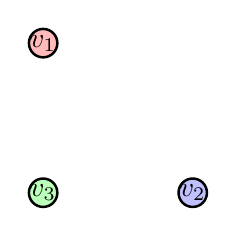
\begin{tikzpicture}[x=0.95cm,y=0.95cm]
  \fill[red!70, fill opacity=0.38] (0.000,2.000) circle[radius=0.19];
  \fill[green!70, fill opacity=0.38] (0.000,0.000) circle[radius=0.19];
  \fill[blue!65, fill opacity=0.38] (2.000,0.000) circle[radius=0.19];
  \draw[black, line width=0.9pt] (0.000,2.000) circle[radius=0.19];
  \draw[black, line width=0.9pt] (0.000,0.000) circle[radius=0.19];
  \draw[black, line width=0.9pt] (2.000,0.000) circle[radius=0.19];
  \node[inner sep=0pt] at (0.000,2.000) {$v_{1}$};
  \node[inner sep=0pt] at (0.000,0.000) {$v_{3}$};
  \node[inner sep=0pt] at (2.000,0.000) {$v_{2}$};
\end{tikzpicture}
